
            \documentclass[a4paper,10pt]{article}
            \usepackage[utf8]{inputenc}
            \usepackage{tikz}
            \usepackage{pifont}
            \usepackage{textcomp}
            % Extrait du paquet fourier.sty
            \newcommand*{\TakeFourierOrnament}[1]{{%
            \fontencoding{U}\fontfamily{futs}\selectfont\char#1}}
            \newcommand*{\decofourleft}{\TakeFourierOrnament{91}}
            \newcommand*{\decofourright}{\TakeFourierOrnament{92}}
            \usepackage[left=1cm,right=1cm,top=1cm,bottom=1cm]{geometry}
            \parindent=0cm
            \newcommand{\tikzscale}{.5}
            \makeatletter
            \newcommand{\simfill}{%
            \leavevmode \cleaders \hb@xt@ .50em{\hss $\sim$\hss }\hfill \kern \z@
            }
            \makeatother
            \begin{document}
            
            
\begin{tikzpicture}[scale=0.25]
            \draw[fill=black] (0,0) rectangle (1,1);
            \end{tikzpicture}\hfill
            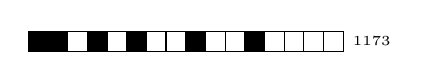
\begin{tikzpicture}[scale=0.25]
            \draw[fill=black] (-1,0) rectangle (0,1);
            \draw[fill=black] (0,0) rectangle (1,1);
                \draw[fill=white] (1,0) rectangle (2,1);
                \draw[fill=black] (2,0) rectangle (3,1);
                \draw[fill=white] (3,0) rectangle (4,1);
                \draw[fill=black] (4,0) rectangle (5,1);
                \draw[fill=white] (5,0) rectangle (6,1);
                \draw[fill=white] (6,0) rectangle (7,1);
                \draw[fill=black] (7,0) rectangle (8,1);
                \draw[fill=white] (8,0) rectangle (9,1);
                \draw[fill=white] (9,0) rectangle (10,1);
                \draw[fill=black] (10,0) rectangle (11,1);
                \draw[fill=white] (11,0) rectangle (12,1);
                \draw[fill=white] (12,0) rectangle (13,1);
                \draw[fill=white] (13,0) rectangle (14,1);
                \draw[fill=white] (14,0) rectangle (15,1);
                \draw (15, .5) node [right] {\tiny1173};
            \end{tikzpicture}
            \hfill
            
\begin{tikzpicture}[scale=0.25]
            \draw[fill=black] (0,0) rectangle (1,1);
            \end{tikzpicture}
            

            \vspace{-.5em}
            \begin{scriptsize}\hfill\textsc{Ne rien écrire ci-dessus.}\hfill\hfill\hfill\textsc{Ne rien écrire ci-dessus.}\hfill\hfil\end{scriptsize}

            

                \vspace{-1em}
                \begin{center}
                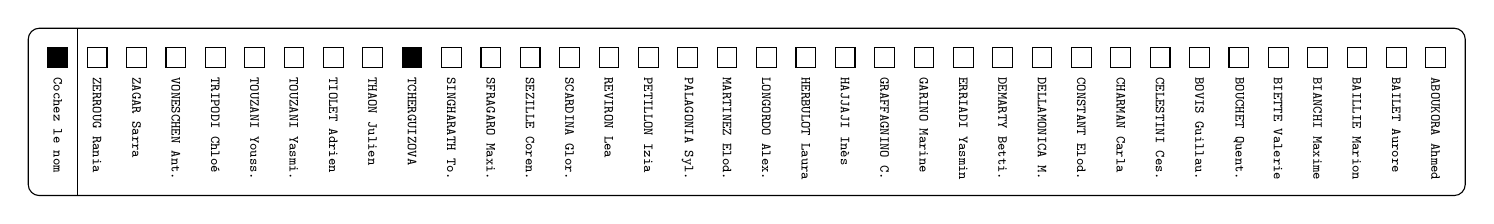
\begin{tikzpicture}[scale=.25]
                \draw [fill=black] (-2,0) rectangle (-1,1) (-1.5,0) node[below] {\tiny\rotatebox{-90}{\texttt{\textbf{Cochez le nom}}}};\draw[fill=white] (0,0) rectangle (1,1) (0.5,0) node[below]
                        {\tiny \rotatebox{-90}{\texttt{ZERROUG Rania}}};\draw[fill=white] (2,0) rectangle (3,1) (2.5,0) node[below]
                        {\tiny \rotatebox{-90}{\texttt{ZAGAR Sarra}}};\draw[fill=white] (4,0) rectangle (5,1) (4.5,0) node[below]
                        {\tiny \rotatebox{-90}{\texttt{VONESCHEN Ant.}}};\draw[fill=white] (6,0) rectangle (7,1) (6.5,0) node[below]
                        {\tiny \rotatebox{-90}{\texttt{TRIPODI Chloé}}};\draw[fill=white] (8,0) rectangle (9,1) (8.5,0) node[below]
                        {\tiny \rotatebox{-90}{\texttt{TOUZANI Youss.}}};\draw[fill=white] (10,0) rectangle (11,1) (10.5,0) node[below]
                        {\tiny \rotatebox{-90}{\texttt{TOUZANI Yasmi.}}};\draw[fill=white] (12,0) rectangle (13,1) (12.5,0) node[below]
                        {\tiny \rotatebox{-90}{\texttt{TIOLET Adrien}}};\draw[fill=white] (14,0) rectangle (15,1) (14.5,0) node[below]
                        {\tiny \rotatebox{-90}{\texttt{THAON Julien}}};\draw[fill=black] (16,0) rectangle (17,1) (16.5,0) node[below]
                        {\tiny \rotatebox{-90}{\texttt{TCHERGUIZOVA}}};\draw[fill=white] (18,0) rectangle (19,1) (18.5,0) node[below]
                        {\tiny \rotatebox{-90}{\texttt{SINGHARATH To.}}};\draw[fill=white] (20,0) rectangle (21,1) (20.5,0) node[below]
                        {\tiny \rotatebox{-90}{\texttt{SFRAGARO Maxi.}}};\draw[fill=white] (22,0) rectangle (23,1) (22.5,0) node[below]
                        {\tiny \rotatebox{-90}{\texttt{SEZILLE Coren.}}};\draw[fill=white] (24,0) rectangle (25,1) (24.5,0) node[below]
                        {\tiny \rotatebox{-90}{\texttt{SCARDINA Glor.}}};\draw[fill=white] (26,0) rectangle (27,1) (26.5,0) node[below]
                        {\tiny \rotatebox{-90}{\texttt{REVIRON Lea}}};\draw[fill=white] (28,0) rectangle (29,1) (28.5,0) node[below]
                        {\tiny \rotatebox{-90}{\texttt{PETILLON Izia}}};\draw[fill=white] (30,0) rectangle (31,1) (30.5,0) node[below]
                        {\tiny \rotatebox{-90}{\texttt{PALAGONIA Syl.}}};\draw[fill=white] (32,0) rectangle (33,1) (32.5,0) node[below]
                        {\tiny \rotatebox{-90}{\texttt{MARTINEZ Elod.}}};\draw[fill=white] (34,0) rectangle (35,1) (34.5,0) node[below]
                        {\tiny \rotatebox{-90}{\texttt{LONGORDO Alex.}}};\draw[fill=white] (36,0) rectangle (37,1) (36.5,0) node[below]
                        {\tiny \rotatebox{-90}{\texttt{HERBULOT Laura}}};\draw[fill=white] (38,0) rectangle (39,1) (38.5,0) node[below]
                        {\tiny \rotatebox{-90}{\texttt{HAJJAJI Inès}}};\draw[fill=white] (40,0) rectangle (41,1) (40.5,0) node[below]
                        {\tiny \rotatebox{-90}{\texttt{GRAFFAGNINO C.}}};\draw[fill=white] (42,0) rectangle (43,1) (42.5,0) node[below]
                        {\tiny \rotatebox{-90}{\texttt{GARINO Marine}}};\draw[fill=white] (44,0) rectangle (45,1) (44.5,0) node[below]
                        {\tiny \rotatebox{-90}{\texttt{ERRIADI Yasmin}}};\draw[fill=white] (46,0) rectangle (47,1) (46.5,0) node[below]
                        {\tiny \rotatebox{-90}{\texttt{DEMARTY Betti.}}};\draw[fill=white] (48,0) rectangle (49,1) (48.5,0) node[below]
                        {\tiny \rotatebox{-90}{\texttt{DELLAMONICA M.}}};\draw[fill=white] (50,0) rectangle (51,1) (50.5,0) node[below]
                        {\tiny \rotatebox{-90}{\texttt{CONSTANT Elod.}}};\draw[fill=white] (52,0) rectangle (53,1) (52.5,0) node[below]
                        {\tiny \rotatebox{-90}{\texttt{CHARMAN Carla}}};\draw[fill=white] (54,0) rectangle (55,1) (54.5,0) node[below]
                        {\tiny \rotatebox{-90}{\texttt{CELESTINI Ces.}}};\draw[fill=white] (56,0) rectangle (57,1) (56.5,0) node[below]
                        {\tiny \rotatebox{-90}{\texttt{BOVIS Guillau.}}};\draw[fill=white] (58,0) rectangle (59,1) (58.5,0) node[below]
                        {\tiny \rotatebox{-90}{\texttt{BOUCHET Quent.}}};\draw[fill=white] (60,0) rectangle (61,1) (60.5,0) node[below]
                        {\tiny \rotatebox{-90}{\texttt{BIETTE Valerie}}};\draw[fill=white] (62,0) rectangle (63,1) (62.5,0) node[below]
                        {\tiny \rotatebox{-90}{\texttt{BIANCHI Maxime}}};\draw[fill=white] (64,0) rectangle (65,1) (64.5,0) node[below]
                        {\tiny \rotatebox{-90}{\texttt{BAILLIE Marion}}};\draw[fill=white] (66,0) rectangle (67,1) (66.5,0) node[below]
                        {\tiny \rotatebox{-90}{\texttt{BAILET Aurore}}};\draw[fill=white] (68,0) rectangle (69,1) (68.5,0) node[below]
                        {\tiny \rotatebox{-90}{\texttt{ABOUKORA Ahmed}}};\draw[rounded corners] (-3,2) rectangle (70, -6.5);
                \draw[] (-0.5,2) -- (-0.5,-6.5);
                \end{tikzpicture}
                \end{center}
                \vspace{-1em}

                
        \simfill
        \vspace{.5em}

        \hfill\hfill 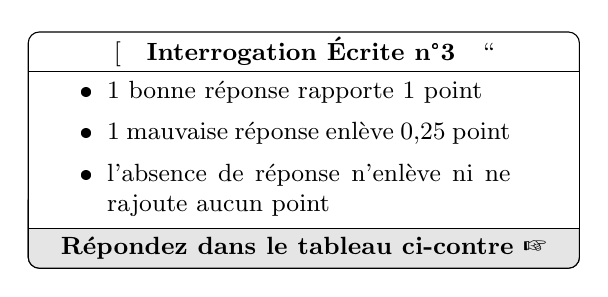
\begin{tikzpicture}[scale=0.5]
                      \draw[rounded corners] (0,1) rectangle (14,-5);
                      \draw[rounded corners,fill=gray!20!white] (0,-3) rectangle (14,-5);
                      \draw[fill=white]  (0,0) rectangle (14,-4);
                      \draw (0,0) -- (14,0) (7,0.5) node {\small\decofourleft\quad\textbf{\textsc{Interrogation Écrite n\textdegree{}3}}\quad\decofourright};
                      \draw (0,0) node [below right] {\small\begin{minipage}{6cm}
                                                        \begin{itemize}
                                                         \item 1 bonne réponse rapporte 1 point
                                                         \item 1 mauvaise réponse enlève 0,25 point
                                                         \item l'absence de réponse n'enlève ni ne rajoute aucun point
                                                        \end{itemize}
                                                       \end{minipage}};

                      \draw (0,-4) -- (14,-4) (7,-4.5) node {\small\textbf{Répondez dans le tableau ci-contre \ding{43}}};


                     \end{tikzpicture}
            \hfill
            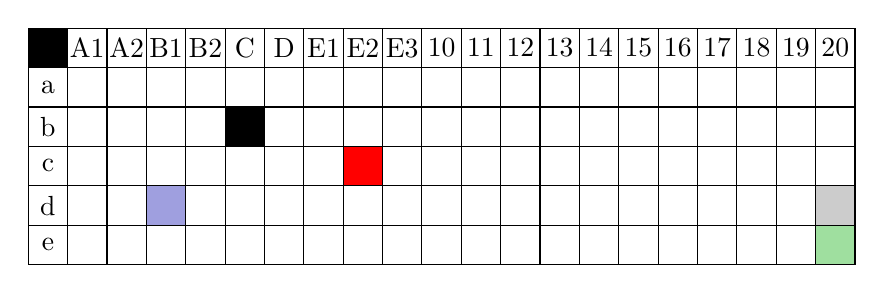
\begin{tikzpicture}[scale=0.5]
            \draw[fill=black] (-1,0) rectangle (0,1);
            \draw (0,0) rectangle (1,1) (0.5,0.5) node {A1};
                \draw (1,0) rectangle (2,1) (1.5,0.5) node {A2};
                \draw (2,0) rectangle (3,1) (2.5,0.5) node {B1};
                \draw (3,0) rectangle (4,1) (3.5,0.5) node {B2};
                \draw (4,0) rectangle (5,1) (4.5,0.5) node {C};
                \draw (5,0) rectangle (6,1) (5.5,0.5) node {D};
                \draw (6,0) rectangle (7,1) (6.5,0.5) node {E1};
                \draw (7,0) rectangle (8,1) (7.5,0.5) node {E2};
                \draw (8,0) rectangle (9,1) (8.5,0.5) node {E3};
                \draw (9,0) rectangle (10,1) (9.5,0.5) node {10};
                \draw (10,0) rectangle (11,1) (10.5,0.5) node {11};
                \draw (11,0) rectangle (12,1) (11.5,0.5) node {12};
                \draw (12,0) rectangle (13,1) (12.5,0.5) node {13};
                \draw (13,0) rectangle (14,1) (13.5,0.5) node {14};
                \draw (14,0) rectangle (15,1) (14.5,0.5) node {15};
                \draw (15,0) rectangle (16,1) (15.5,0.5) node {16};
                \draw (16,0) rectangle (17,1) (16.5,0.5) node {17};
                \draw (17,0) rectangle (18,1) (17.5,0.5) node {18};
                \draw (18,0) rectangle (19,1) (18.5,0.5) node {19};
                \draw (19,0) rectangle (20,1) (19.5,0.5) node {20};
                
                \draw (-1,0) rectangle (0,-1) (-0.5,-0.5) node {a};
                \draw [] (0,0) rectangle (1,-1);
                    \draw [] (1,0) rectangle (2,-1);
                    \draw [] (2,0) rectangle (3,-1);
                    \draw [] (3,0) rectangle (4,-1);
                    \draw [] (4,0) rectangle (5,-1);
                    \draw [] (5,0) rectangle (6,-1);
                    \draw [] (6,0) rectangle (7,-1);
                    \draw [] (7,0) rectangle (8,-1);
                    \draw [] (8,0) rectangle (9,-1);
                    \draw [] (9,0) rectangle (10,-1);
                    \draw [] (10,0) rectangle (11,-1);
                    \draw [] (11,0) rectangle (12,-1);
                    \draw [] (12,0) rectangle (13,-1);
                    \draw [] (13,0) rectangle (14,-1);
                    \draw [] (14,0) rectangle (15,-1);
                    \draw [] (15,0) rectangle (16,-1);
                    \draw [] (16,0) rectangle (17,-1);
                    \draw [] (17,0) rectangle (18,-1);
                    \draw [] (18,0) rectangle (19,-1);
                    \draw [] (19,0) rectangle (20,-1);
                    
                \draw (-1,-1) rectangle (0,-2) (-0.5,-1.5) node {b};
                \draw [] (0,-1) rectangle (1,-2);
                    \draw [] (1,-1) rectangle (2,-2);
                    \draw [] (2,-1) rectangle (3,-2);
                    \draw [] (3,-1) rectangle (4,-2);
                    \draw [fill=black] (4,-1) rectangle (5,-2);
                    \draw [] (5,-1) rectangle (6,-2);
                    \draw [] (6,-1) rectangle (7,-2);
                    \draw [] (7,-1) rectangle (8,-2);
                    \draw [] (8,-1) rectangle (9,-2);
                    \draw [] (9,-1) rectangle (10,-2);
                    \draw [] (10,-1) rectangle (11,-2);
                    \draw [] (11,-1) rectangle (12,-2);
                    \draw [] (12,-1) rectangle (13,-2);
                    \draw [] (13,-1) rectangle (14,-2);
                    \draw [] (14,-1) rectangle (15,-2);
                    \draw [] (15,-1) rectangle (16,-2);
                    \draw [] (16,-1) rectangle (17,-2);
                    \draw [] (17,-1) rectangle (18,-2);
                    \draw [] (18,-1) rectangle (19,-2);
                    \draw [] (19,-1) rectangle (20,-2);
                    
                \draw (-1,-2) rectangle (0,-3) (-0.5,-2.5) node {c};
                \draw [] (0,-2) rectangle (1,-3);
                    \draw [] (1,-2) rectangle (2,-3);
                    \draw [] (2,-2) rectangle (3,-3);
                    \draw [] (3,-2) rectangle (4,-3);
                    \draw [] (4,-2) rectangle (5,-3);
                    \draw [] (5,-2) rectangle (6,-3);
                    \draw [] (6,-2) rectangle (7,-3);
                    \draw [fill=red] (7,-2) rectangle (8,-3);
                    \draw [] (8,-2) rectangle (9,-3);
                    \draw [] (9,-2) rectangle (10,-3);
                    \draw [] (10,-2) rectangle (11,-3);
                    \draw [] (11,-2) rectangle (12,-3);
                    \draw [] (12,-2) rectangle (13,-3);
                    \draw [] (13,-2) rectangle (14,-3);
                    \draw [] (14,-2) rectangle (15,-3);
                    \draw [] (15,-2) rectangle (16,-3);
                    \draw [] (16,-2) rectangle (17,-3);
                    \draw [] (17,-2) rectangle (18,-3);
                    \draw [] (18,-2) rectangle (19,-3);
                    \draw [] (19,-2) rectangle (20,-3);
                    
                \draw (-1,-3) rectangle (0,-4) (-0.5,-3.5) node {d};
                \draw [] (0,-3) rectangle (1,-4);
                    \draw [] (1,-3) rectangle (2,-4);
                    \draw [fill=blue!50!gray!50!white] (2,-3) rectangle (3,-4);
                    \draw [] (3,-3) rectangle (4,-4);
                    \draw [] (4,-3) rectangle (5,-4);
                    \draw [] (5,-3) rectangle (6,-4);
                    \draw [] (6,-3) rectangle (7,-4);
                    \draw [] (7,-3) rectangle (8,-4);
                    \draw [] (8,-3) rectangle (9,-4);
                    \draw [] (9,-3) rectangle (10,-4);
                    \draw [] (10,-3) rectangle (11,-4);
                    \draw [] (11,-3) rectangle (12,-4);
                    \draw [] (12,-3) rectangle (13,-4);
                    \draw [] (13,-3) rectangle (14,-4);
                    \draw [] (14,-3) rectangle (15,-4);
                    \draw [] (15,-3) rectangle (16,-4);
                    \draw [] (16,-3) rectangle (17,-4);
                    \draw [] (17,-3) rectangle (18,-4);
                    \draw [] (18,-3) rectangle (19,-4);
                    \draw [fill=black!20!white] (19,-3) rectangle (20,-4);
                    
                \draw (-1,-4) rectangle (0,-5) (-0.5,-4.5) node {e};
                \draw [] (0,-4) rectangle (1,-5);
                    \draw [] (1,-4) rectangle (2,-5);
                    \draw [] (2,-4) rectangle (3,-5);
                    \draw [] (3,-4) rectangle (4,-5);
                    \draw [] (4,-4) rectangle (5,-5);
                    \draw [] (5,-4) rectangle (6,-5);
                    \draw [] (6,-4) rectangle (7,-5);
                    \draw [] (7,-4) rectangle (8,-5);
                    \draw [] (8,-4) rectangle (9,-5);
                    \draw [] (9,-4) rectangle (10,-5);
                    \draw [] (10,-4) rectangle (11,-5);
                    \draw [] (11,-4) rectangle (12,-5);
                    \draw [] (12,-4) rectangle (13,-5);
                    \draw [] (13,-4) rectangle (14,-5);
                    \draw [] (14,-4) rectangle (15,-5);
                    \draw [] (15,-4) rectangle (16,-5);
                    \draw [] (16,-4) rectangle (17,-5);
                    \draw [] (17,-4) rectangle (18,-5);
                    \draw [] (18,-4) rectangle (19,-5);
                    \draw [fill=green!50!gray!50!white] (19,-4) rectangle (20,-5);
                    
\end{tikzpicture}
\hfill\hfill\hfil
\end{document}
